% Checked against master: backend/orchestrator/service.py, backend/satra/live_pipeline.py,
% backend/satra/api.py, backend/sable/analyzer.py.
% ======================================================================
% (7) Ch 5 "Process / Behavior Design": put FIRST in the section (system level)
% ======================================================================
\begin{figure}[htbp]
\centering
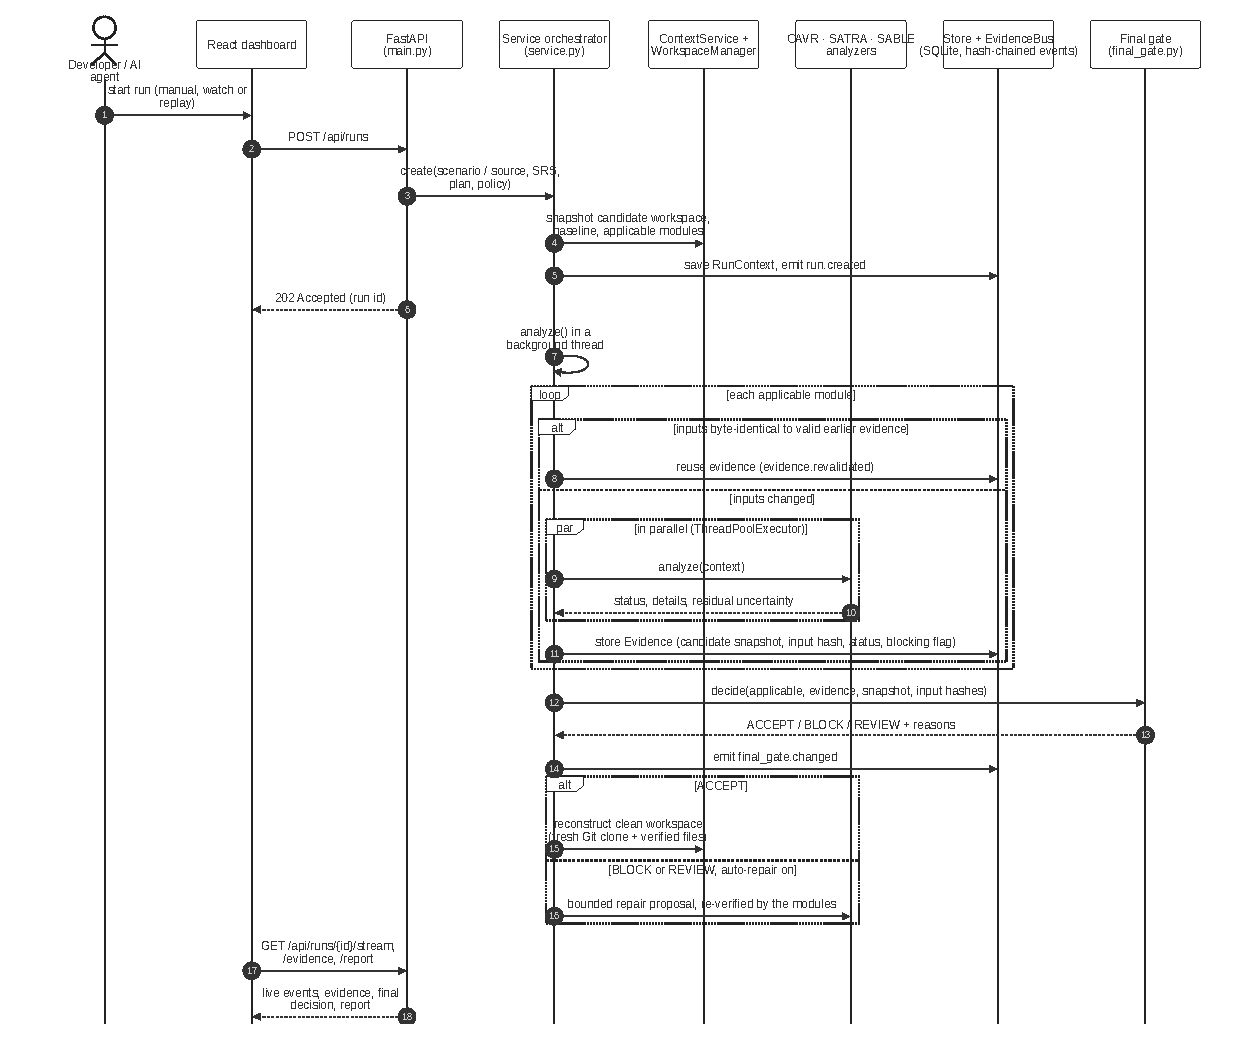
\includegraphics[width=\textwidth]{figures/diagrams/system-sequence.pdf}
\caption{End-to-end sequence of an ASENT assurance run: API, orchestrator, parallel module analyzers, evidence store and shared final gate (\texttt{backend/orchestrator/service.py}).}
\label{fig:asent-system-sequence}
\end{figure}

Figure~\ref{fig:asent-system-sequence} shows one assurance run across the whole system. \texttt{POST /api/runs} makes the orchestrator snapshot the candidate workspace and work out which modules apply; the API returns at once and the analysis continues in a background thread. For each applicable module, evidence whose inputs are byte-identical to earlier valid evidence is reused; otherwise the CAVR, SATRA-RV and SABLE analyzers run in parallel, and each result is stored as evidence bound to the candidate snapshot and the module's input hash, with every step recorded as a hash-chained event. The final gate then decides \texttt{ACCEPT}, \texttt{BLOCK} or \texttt{REVIEW}; on \texttt{ACCEPT} a clean workspace is reconstructed from a fresh Git clone plus the verified files, and on \texttt{BLOCK} or \texttt{REVIEW} an optional bounded repair is proposed and verified again by the modules. The dashboard follows the run through the stream, evidence and report endpoints.

% ======================================================================
% (8)+(9) SATRA-RV (Sheharyar): Ch 5 "Process / Behavior Design" or next to Figure 6.7
% ======================================================================
\begin{figure}[htbp]
\centering
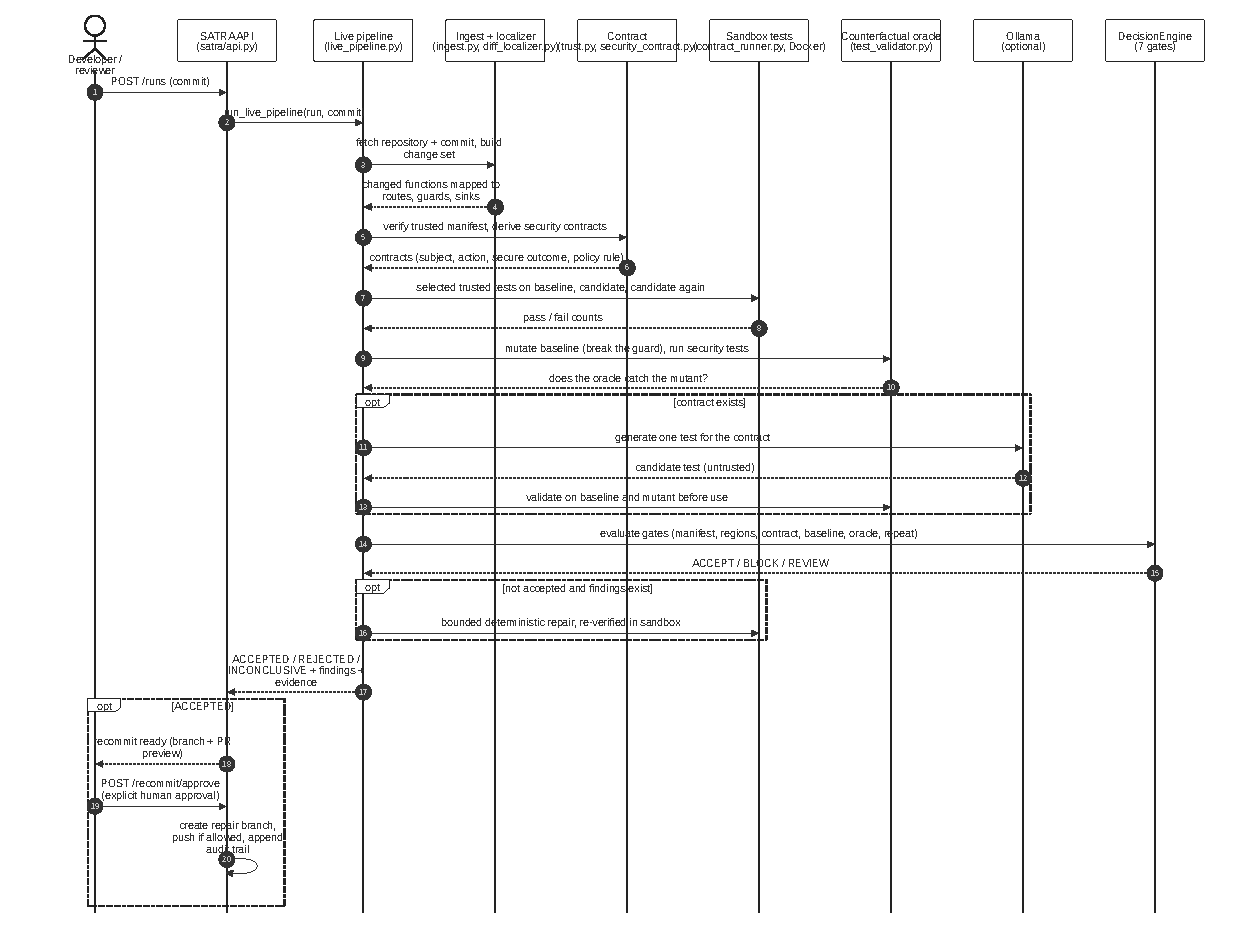
\includegraphics[width=\textwidth]{figures/diagrams/satra-sequence.pdf}
\caption{Sequence of a SATRA-RV live run (\texttt{backend/satra/live\_pipeline.py}) from commit ingestion to the decision and the human-approved recommit.}
\label{fig:satra-sequence}
\end{figure}

\begin{figure}[htbp]
\centering
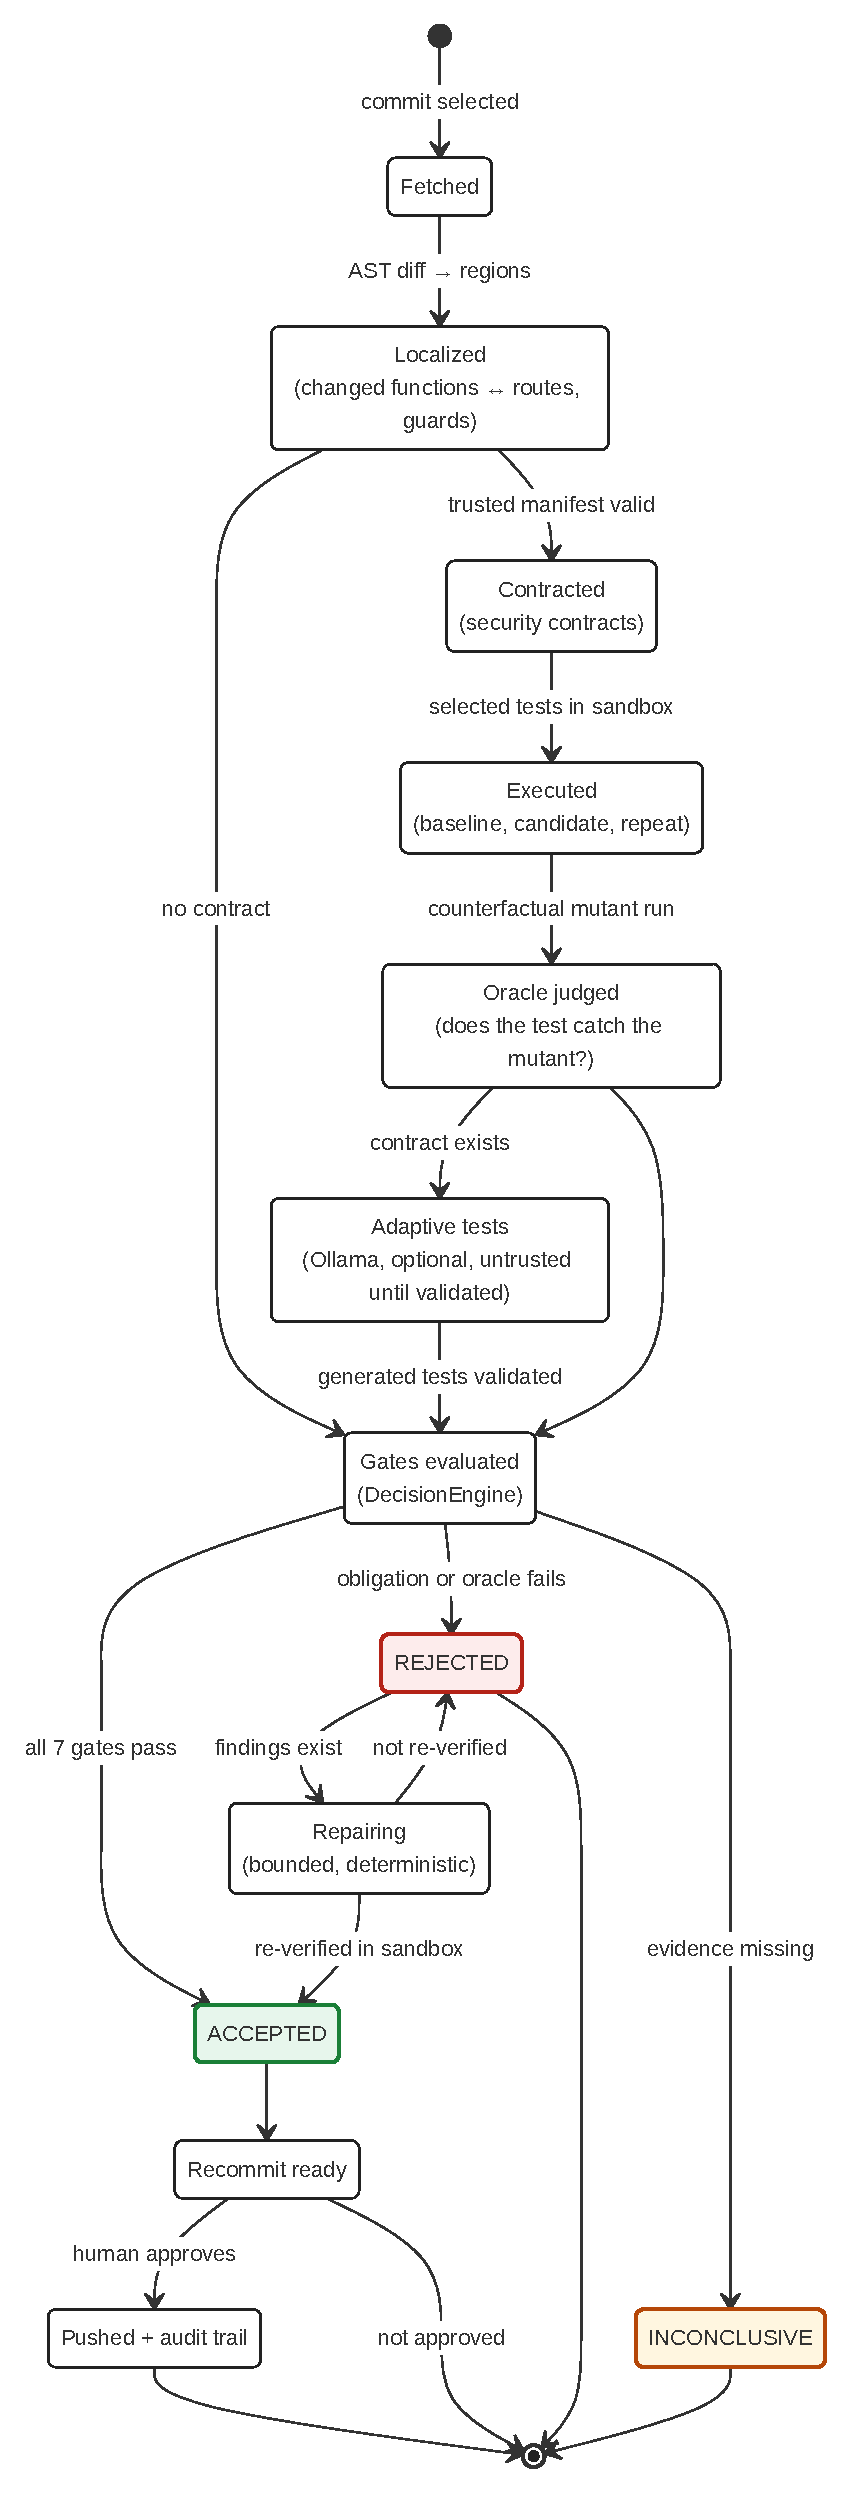
\includegraphics[height=0.8\textheight]{figures/diagrams/satra-state.pdf}
\caption{States of a SATRA-RV run. A repair is only accepted after re-verification in the sandbox, and a recommit is only pushed after explicit human approval.}
\label{fig:satra-state}
\end{figure}

Figures~\ref{fig:satra-sequence} and~\ref{fig:satra-state} show how SATRA-RV judges an application-code change. The commit is fetched and its changed functions are mapped to routes, guards and sinks by AST localization. Security contracts are derived only when the trusted manifest is valid, and the selected trusted tests run in the sandbox on the baseline, the candidate and the candidate again. The counterfactual oracle deliberately breaks the guard in a copy of the baseline and checks that the security tests catch it, so a weak test cannot produce a false pass. Tests generated by Ollama are optional and untrusted until they pass the same validation. The decision engine evaluates seven gates and gives \texttt{ACCEPTED}, \texttt{REJECTED} or \texttt{INCONCLUSIVE}; a rejected run with findings may receive a bounded deterministic repair that counts only after re-verification. An accepted repair is offered as a recommit and is pushed only after an explicit human approval, which is recorded in the audit trail.

% ======================================================================
% (10)+(11) SABLE (Ali): Ch 5 "Process / Behavior Design", after Figure 5.2 text
% ======================================================================
\begin{figure}[htbp]
\centering
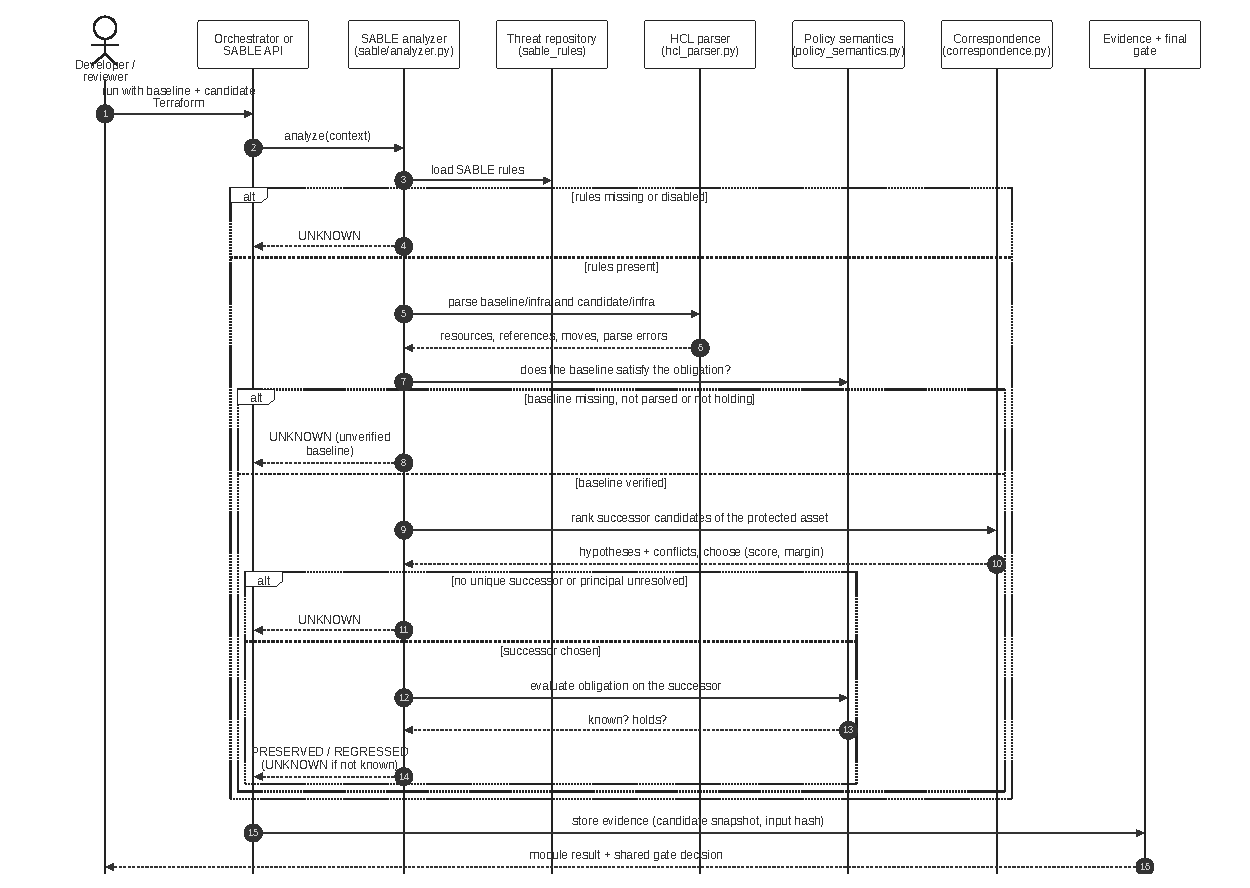
\includegraphics[width=\textwidth]{figures/diagrams/sable-sequence.pdf}
\caption{Sequence of a SABLE analysis (\texttt{backend/sable/analyzer.py}): rules, HCL parsing, baseline verification, successor correspondence and projected authorization.}
\label{fig:sable-sequence}
\end{figure}

\begin{figure}[htbp]
\centering
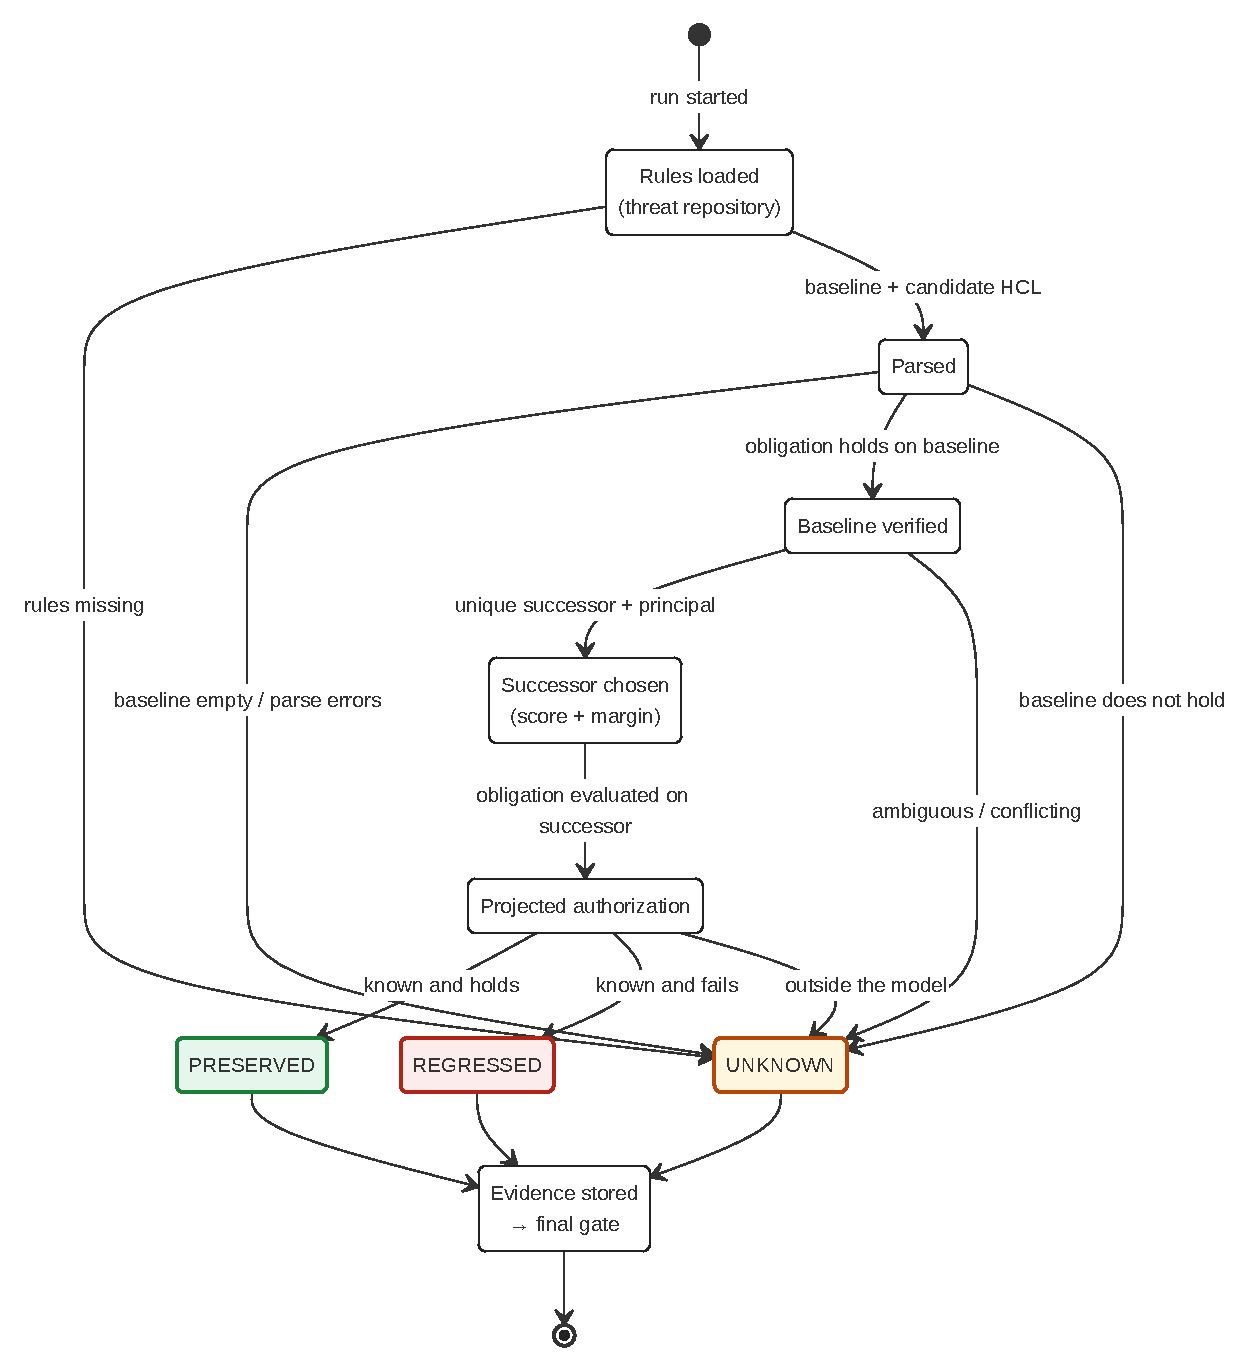
\includegraphics[width=0.85\textwidth]{figures/diagrams/sable-state.pdf}
\caption{States of a SABLE analysis. Every path that cannot establish the obligation ends in \texttt{UNKNOWN}; all results are stored as evidence for the final gate.}
\label{fig:sable-state}
\end{figure}

Figures~\ref{fig:sable-sequence} and~\ref{fig:sable-state} show the order in which SABLE establishes its result. The SABLE rules are loaded from the threat repository, and both Terraform trees are parsed. The registered obligation must first hold on the trusted baseline; only then are successor candidates of the protected asset ranked, and a successor is accepted only with a sufficient score and margin and an unambiguous principal. The obligation is then evaluated on that successor: \texttt{PRESERVED} when it is known to hold, \texttt{REGRESSED} when it is known to fail, and \texttt{UNKNOWN} whenever rules, baseline, correspondence or policy semantics are insufficient, so uncertainty is never reported as preserved.

% ======================================================================
% (12) Ch 5 "Domain Model": CAVR domain model, after the SABLE domain model (Figure 5.4)
% ======================================================================
\begin{figure}[htbp]
\centering
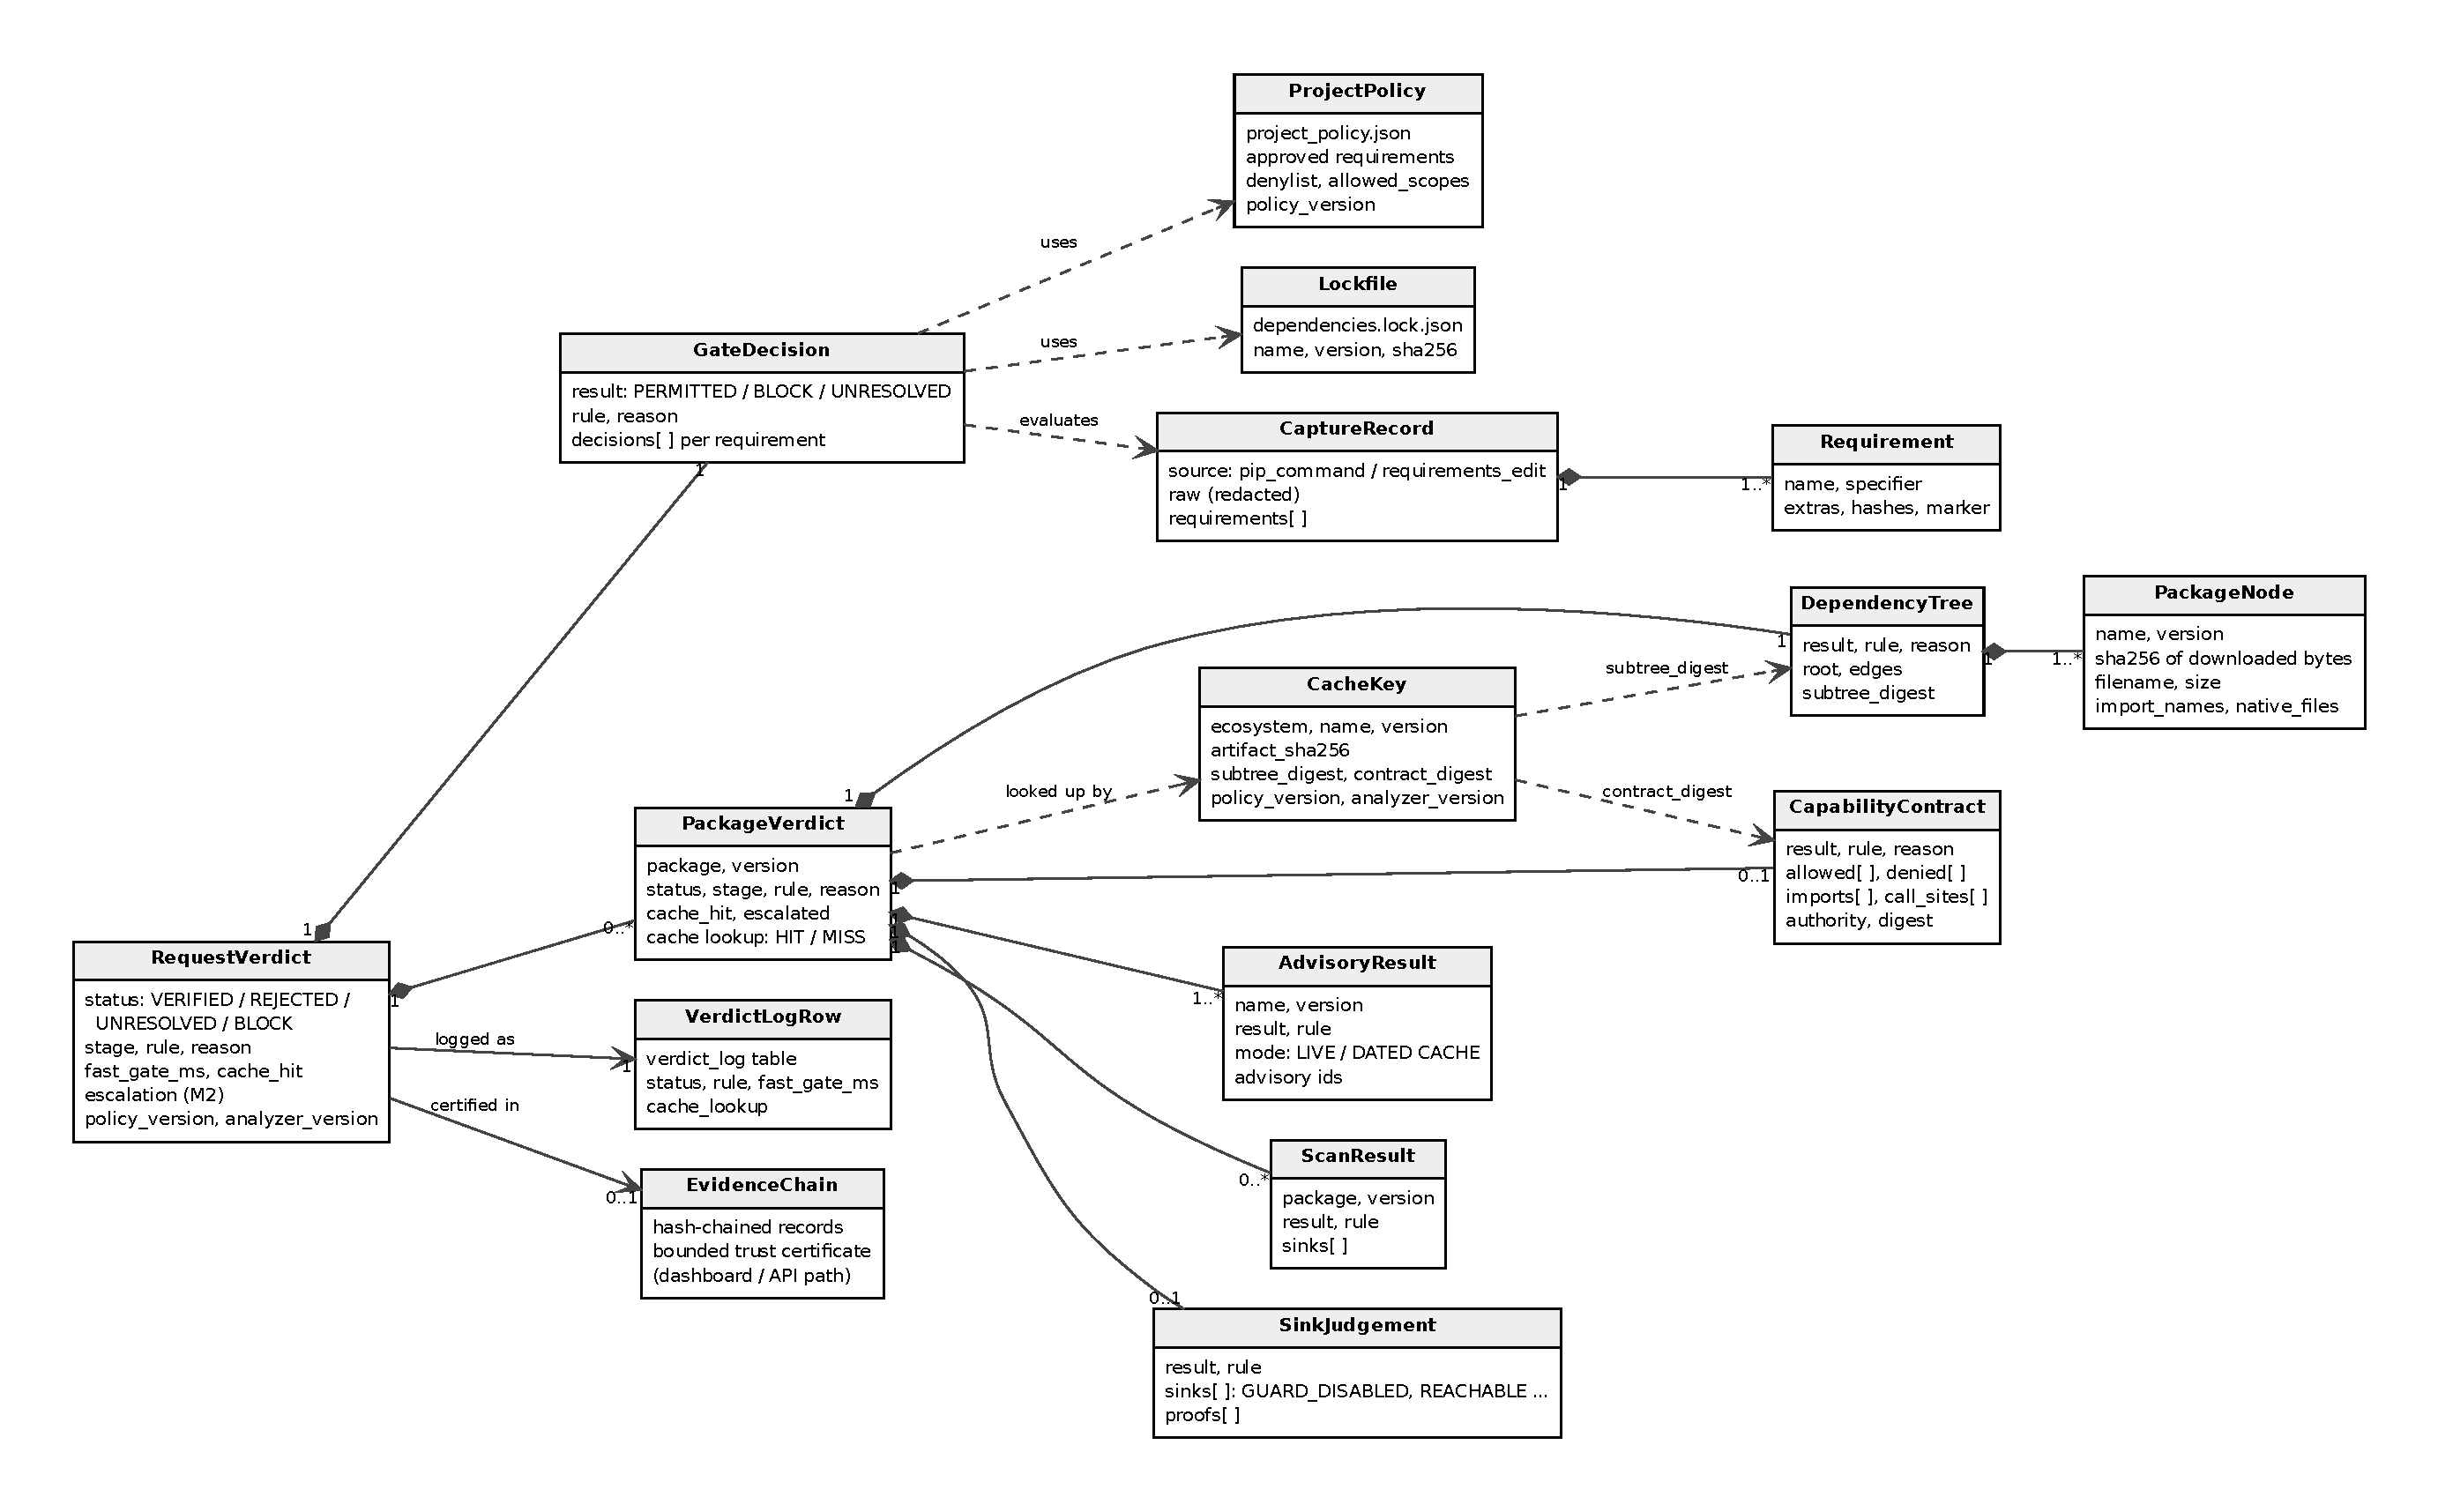
\includegraphics[width=\textwidth]{figures/diagrams/cavr-domain.pdf}
\caption{CAVR domain model: the records produced by \texttt{verify\_request} (\texttt{backend/cavr/pipeline.py}) and how they compose into a request verdict. Filled diamonds are composition; dashed arrows are dependencies.}
\label{fig:cavr-domain-model}
\end{figure}

Figure~\ref{fig:cavr-domain-model} shows the data CAVR works with. A \emph{capture record} holds the requested requirements; the \emph{gate decision} evaluates it against the project policy and the lockfile. Each permitted requirement produces a \emph{package verdict} that is composed of the evidence of every stage: the dependency tree with the SHA-256 of every downloaded wheel, the capability contract inferred from the project's call sites, one advisory result per package of the tree, the scan results and the sink judgement. The \emph{cache key} is built from eight fields, two of which are the subtree digest and the contract digest, so any change to the artifact, its dependencies, the project's use of the package, the policy or the analyzer leads to a new analysis. Every stage result has the same shape (\texttt{result}, \texttt{rule}, \texttt{reason}), which is what lets the request verdict name the exact stage and rule that decided it. Each request verdict is written to the verdict log, and from the dashboard it is also recorded in the hash-chained evidence and its certificate.
